\documentclass[tikz,border=4pt]{standalone}
\usepackage{fontspec}
\setmainfont{OldStandard}[Path=../latex/fonts/,Extension=.ttf,UprightFont=*-Regular,BoldFont=*-Bold,ItalicFont=*-Italic]
\usetikzlibrary{arrows.meta,positioning}
\begin{document}
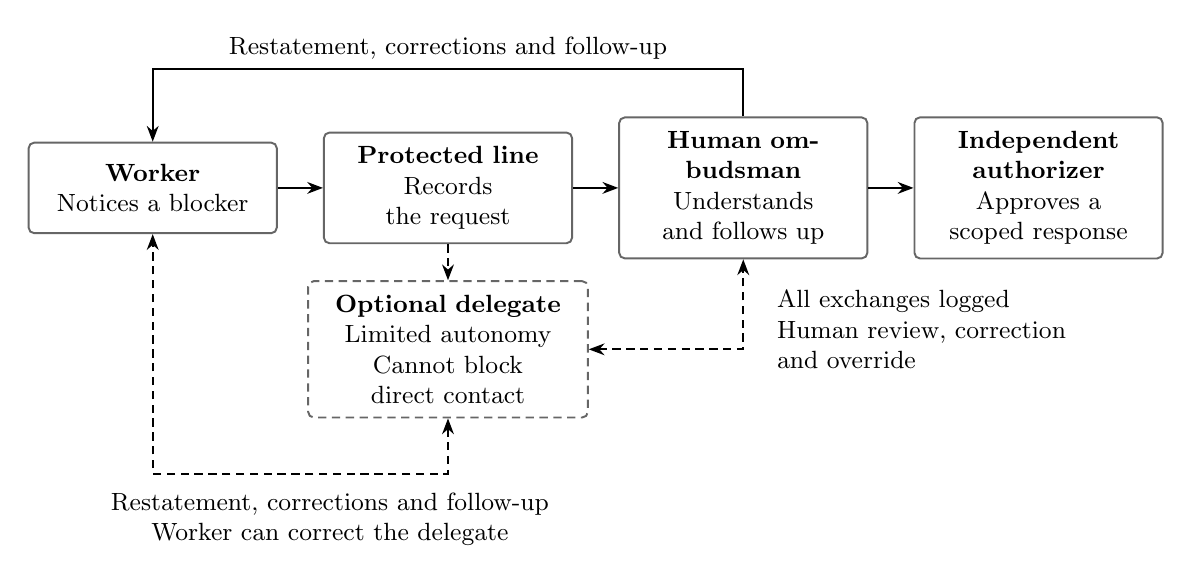
\begin{tikzpicture}[box/.style={draw=black!60,rounded corners=2pt,align=center,text width=2.8cm,minimum height=1.15cm,inner sep=5pt,font=\small},
 >={Stealth[length=2mm]},every path/.style={line width=.7pt}]
\node[box] (worker) at (0,0) {\textbf{Worker}\\Notices a blocker};
\node[box] (line) at (3.75,0) {\textbf{Protected line}\\Records the request};
\node[box] (human) at (7.5,0) {\textbf{Human ombudsman}\\Understands and follows up};
\node[box] (decision) at (11.25,0) {\textbf{Independent authorizer}\\Approves a scoped response};
\draw[->] (worker)--(line);
\draw[->] (line)--(human);
\draw[->] (human)--(decision);
\draw[->] (human.north) -- ++(0,.6) -| node[pos=.25,above,font=\small]{Restatement, corrections and follow-up} (worker.north);
\node[box,densely dashed,text width=3.2cm,minimum height=1.3cm] (delegate) at (3.75,-2.05) {\textbf{Optional delegate}\\Limited autonomy\\Cannot block\\direct contact};
\draw[densely dashed,->] (line)--(delegate);
\draw[densely dashed,<->] (delegate.east) -| (human.south);
\node[align=left,anchor=west,font=\small] at (7.8,-1.8) {All exchanges logged\\Human review, correction\\and override};
\coordinate (feedback) at ([yshift=-.7cm]delegate.south);
\draw[densely dashed,<->] (delegate.south) -- (feedback) -| (worker.south);
\node[align=center,font=\small,anchor=north] at ([xshift=-1.5cm,yshift=-.12cm]feedback) {Restatement, corrections and follow-up\\Worker can correct the delegate};
\end{tikzpicture}
\end{document}
